\documentclass{article}

\renewcommand{\thesection}{}
\renewcommand{\thesubsection}{\arabic{section}.\arabic{subsection}}
\makeatletter
\def\@seccntformat#1{\csname #1ignore\expandafter\endcsname\csname the#1\endcsname\quad}
\let\sectionignore\@gobbletwo
\let\latex@numberline\numberline
\def\numberline#1{\if\relax#1\relax\else\latex@numberline{#1}\fi}
\makeatother

\usepackage[utf8]{inputenc}

\title{Exercício Introdução}
\author{Gustavo Higuchi}
\date{Agosto 2016}

\usepackage{natbib}
\usepackage{graphicx}

\begin{document}

\maketitle
\section{Resposta 1 }
Quanto que um carro percorre, em km, por quanto ele cosome, por litro de combustível, se a taxa for alta, o carro será mais eficiente.
Ou quanto que uma fábrica desperdiça um certo material ao produzir um objeto, se a taxa for pequena, a fábrica será mais eficiente.

\section{Resposta 2}

Sendo \[f(x)=8*n^2\] e \[g(x)=64*n*log_2(n)\], o ponto de intersecção onde as funções se encontram
e g(x) passa a ser menor que f(x) é 44, como mostra a figura.

\begin{figure}[h!]
\centering
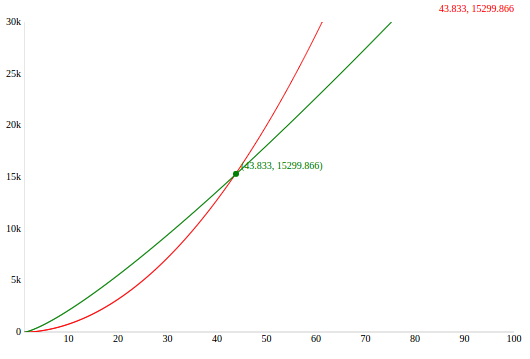
\includegraphics[scale=0.4]{ex_02.png}
\caption{Ponto de interseção entre f(x) e g(x)}
\label{fig:univerise}
\end{figure}

Figura gerada atraves de index.html, disponível em \url{https://github.com/manauera/exercios-analise-alg/tree/master/ex_introducao} 

\section{Resposta 3}

Depois de n=20 já basta.

\begin{figure}[h!]
\centering
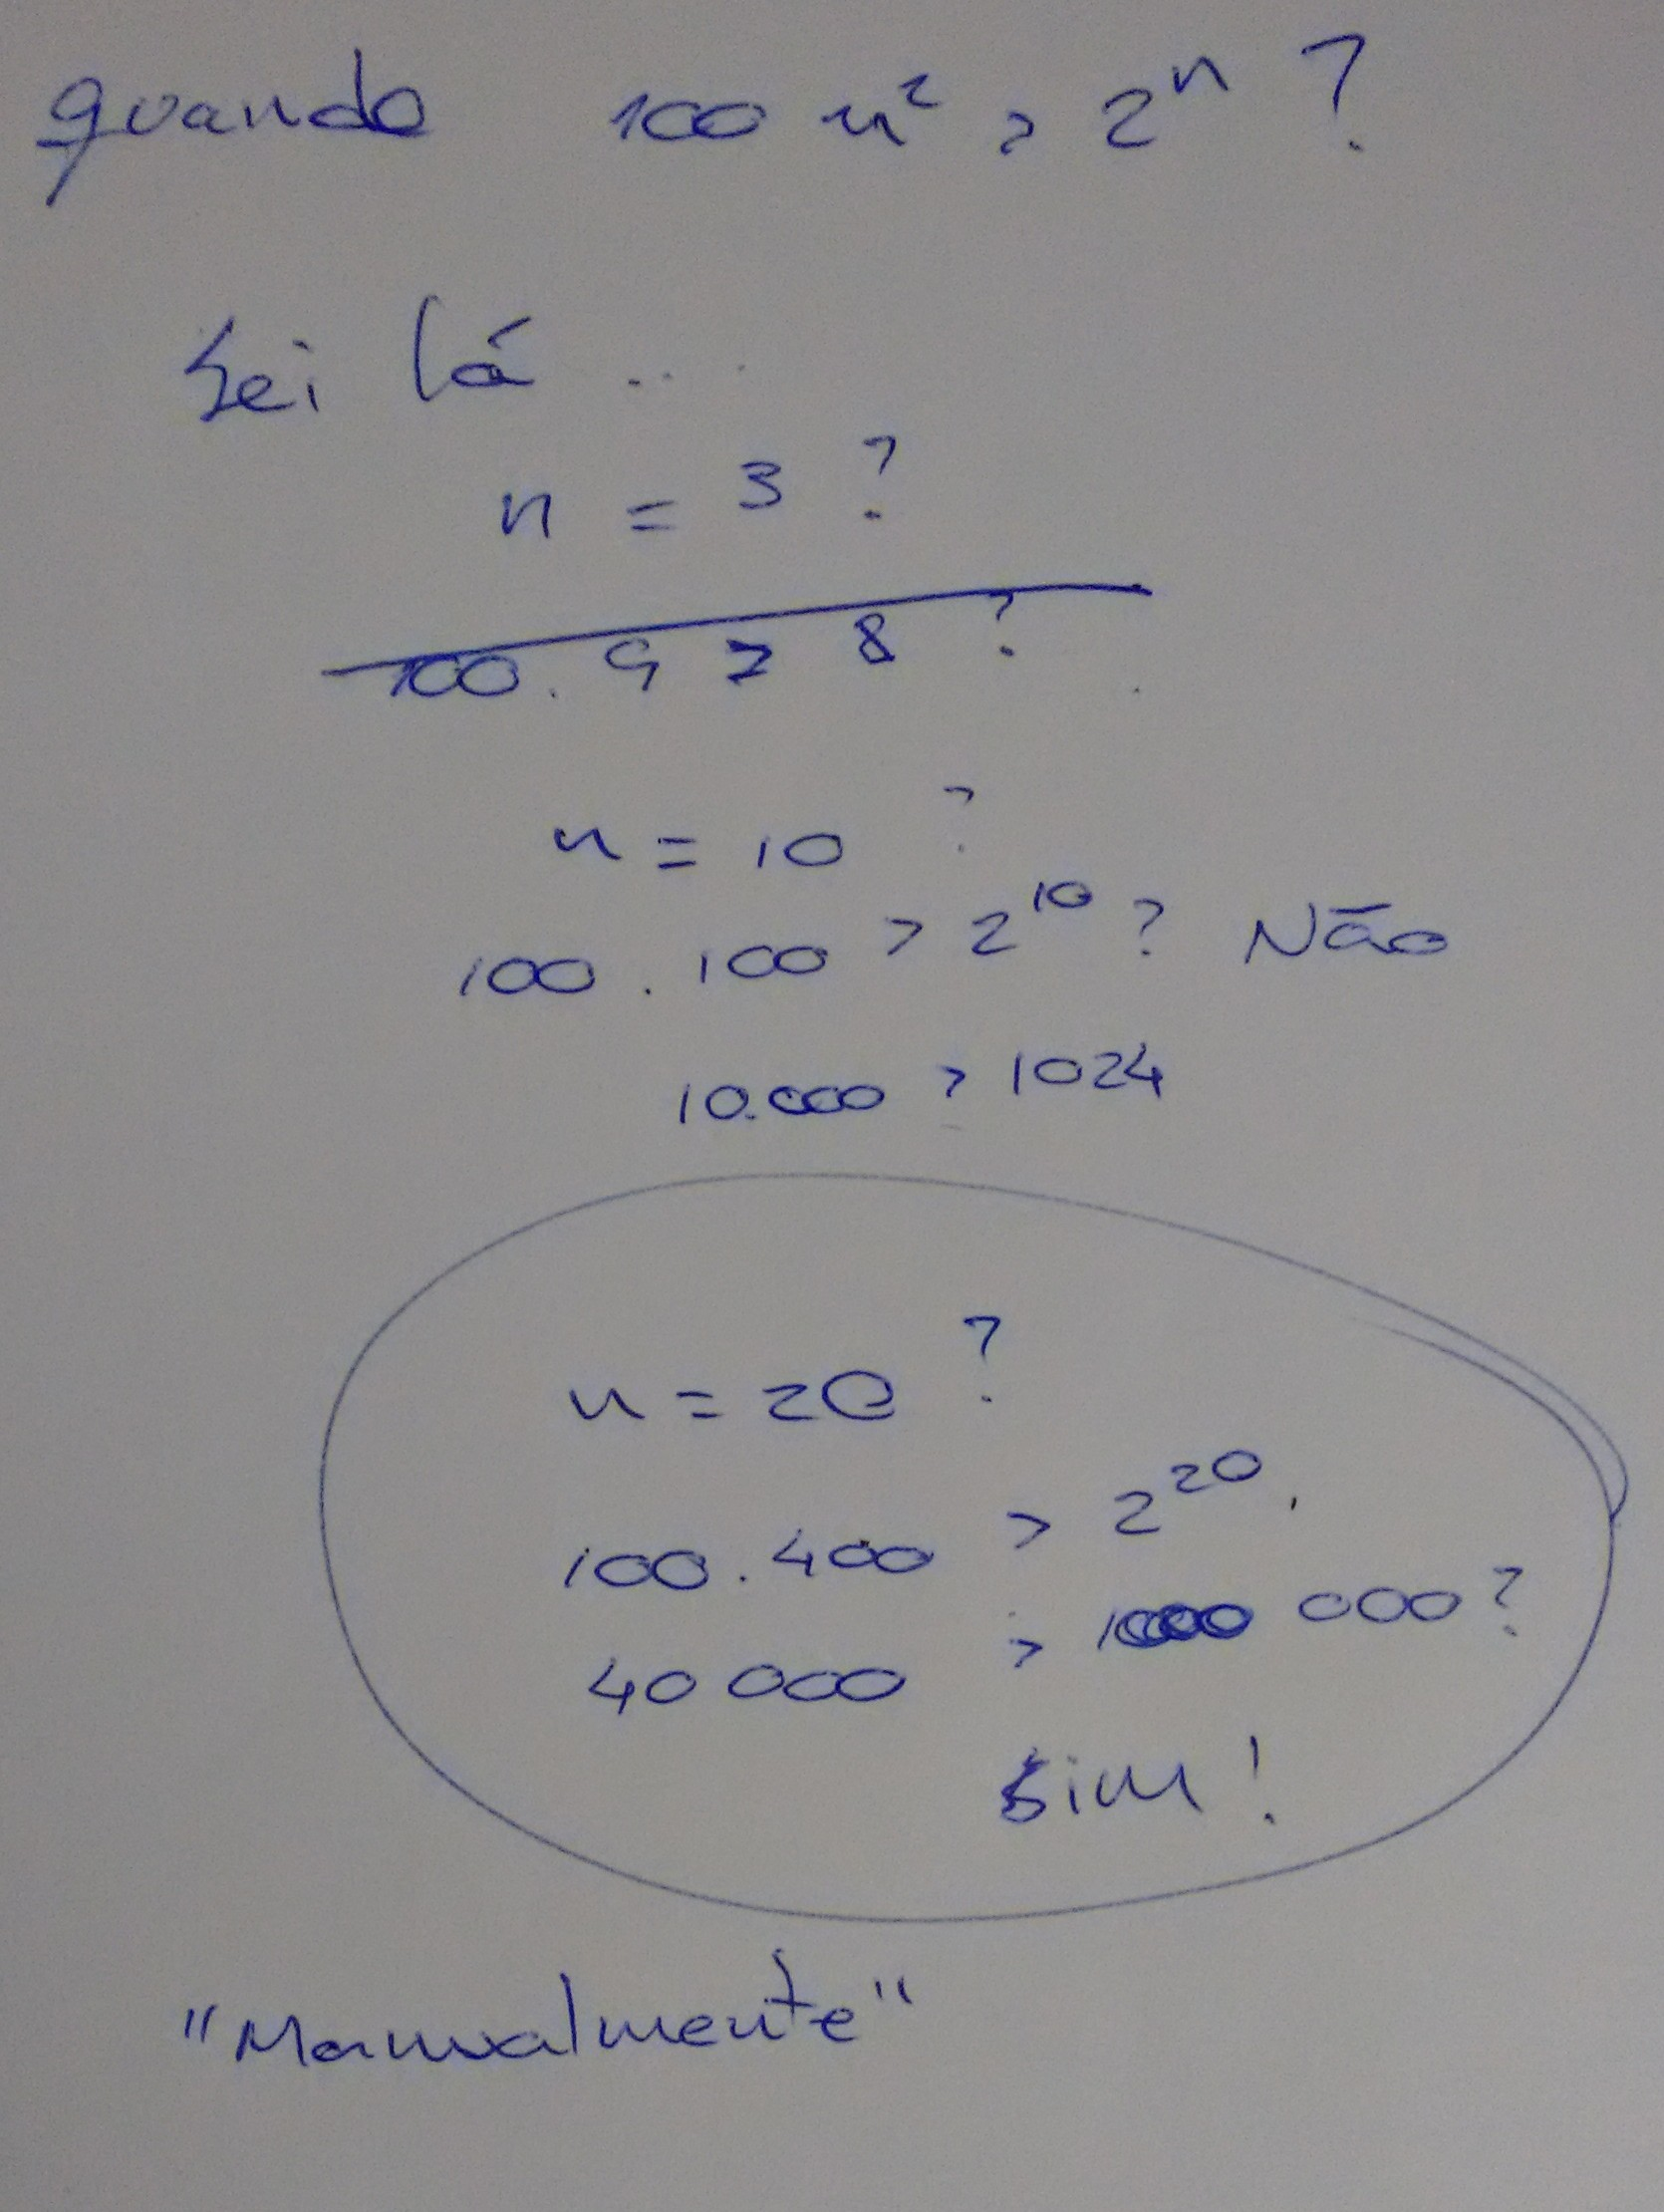
\includegraphics[scale=0.15]{ex_03.jpg}
\caption{Manualmente encontrado}
\label{fig:univerise}
\end{figure}

\end{document}
